\documentclass[15pt,a4paper]{article}

%use the english line for english reports
%usepackage[english]{babel}
\usepackage[portuguese]{babel}
\usepackage[utf8]{inputenc}
\usepackage{indentfirst}
\usepackage{graphicx}
\usepackage{verbatim}
\usepackage{subfig}
\usepackage{float}

\begin{document}

\setlength{\textwidth}{16cm}
\setlength{\textheight}{22cm}


%************************************************************************************************
%************************************************************************************************

\title{
	\Huge\textbf{Breakthrough}
	\linebreak\linebreak\linebreak
	\Large\textbf{Relatório Intercalar}
	\linebreak\linebreak
	
\includegraphics[height=6cm, width=7cm]{feup.pdf}
	\linebreak \linebreak
	\Large{Mestrado Integrado em Engenharia Informática e Computação}
	\linebreak\linebreak
	\Large{Programação em Lógica}\linebreak
}


\author{\textbf{Grupo xx:}
\\ João Guedes - 070509043
\\ João Henriques - 110509026
\\\linebreak\linebreak \\
 \\ Faculdade de Engenharia da Universidade do Porto
\\ Rua Roberto Frias, s\/n, 4200-465 Porto, Portugal
\linebreak\linebreak\linebreak
\linebreak\linebreak\vspace{1cm}}
\date{Setembro de 2011}
\maketitle
\thispagestyle{empty}



%************************************************************************************************
%************************************************************************************************


\section*{Resumo}

% Descrever muito sumariamente o trabalho. Deve ser suficiente para o leitor decidir se lê ou não o resto do relatório.
% Não deve incluir nenhuma referência ao facto de ser feito no âmbito de uma cadeira.



O \textit{Breakthrough} é um jogo de tabuleiro tradicional semelhante às damas, premiado e com um conjunto de regras muito simples e acessível.

A implementação pretendida irá oferecer três modos de jogo - ``Humano/Humano", ``Humano/Computador" e ``Computador/Computador" - sendo que o Computador terá vários níveis
de dificuldade.

Recorreremos à linguagem de programação \textit{ProLog} para o fazer, e a \textit{C++}  para o módulo de visualização gráfico do jogo.



%************************************************************************************************
%************************************************************************************************
\newpage


\tableofcontents

%************************************************************************************************
%************************************************************************************************

%************************************************************************************************
%************************************************************************************************
\newpage


\section{Introdução}

% Descrever os objectivos e motivação do trabalho. Não deve incluir nenhuma referência ao facto de ser feito no âmbito de uma cadeira.
% Último parágrafo deve indicar a estrutura do relatório.
% Devem ser incluídas referências bibliográficas correctas e completas (consultar os docentes em caso de dúvida). Páginas da wikipedia não são consideradas referências válidas \cite{CodigoSite, %CodigoLivro}.
% Todas as figuras devem ser referidas no texto. %\ref{fig:codigoFigura}



Este trabalho tem como principal motivação a consolidação do nosso conhecimento em ProLog, visto que o paradigma de programação é totalmente diferente daquele a que temos vindo a estar habituados ao longo do curso.

Por ser menos exigente e mais exequível dados os nossos conhecimentos, começaremos por implementar o modo ``Humano/Humano" através de regras lógicas.

Seguidamente recorreremos a algoritmos de inteligência artificial e à teoria dos jogos para implementar os modos que envolvam o Computador.


Escolhemos este trabalho porque gostamos da sua simplicidade e fluidez, e apesar de não ter um conjunto de regras muito vasto, é um jogo com potencial estratégico. 
Se o oponente não estiver atento, é capaz de ser vencido muito rapidamente.

De notar que apesar da nossa implementação consistir num tabuleiro convencional de ``8x8", o \textit{Breakthrough} pode ser jogado com outras configurações, como tabuleiros ``7x7" ou tabuleiros não-quadrados

%Código para inserção de figuras
%\begin{figure}[h!]
%\begin{center}
%escolher entre uma das seguintes três linhas:
%\includegraphics[height=20cm,width=15cm]{path relativo da imagem}
%\includegraphics[scale=0.5]{path relativo da imagem}
%\includegraphics{path relativo da imagem}
%\caption{legenda da figura}
%\label{fig:codigoFigura}
%\end{center}
%\end{figure}

%Ajuda:

%\textit{Para escrever em itálico}

%\textbf{Para escrever em negrito}

%Para escrever em letra normal

%``Para escrever texto entre aspas''

%Para fazer parágrafo, deixar uma linha em branco.

%Como fazer bullet points:

%\begin{itemize}
%\item Item1
%\item Item2
%\end{itemize}

%Como enumerar itens:

%\begin{enumerate}
%\item Item 1
%\end{enumerate}

%\begin{quote}``Isto é uma citação''\end{quote}

%************************************************************************************************
%************************************************************************************************

\newpage

\section{Descrição do Problema}
%Descrever sucintamente o jogo, a sua história e, principalmente, as suas regras. Devem ser criadas/utilizadas imagens apropriadas para explicar o funcionamento do jogo.

O \textit{Breakthrough} foi criado no ano 2000 por \textit{Dan Troyka}  e disponibilizado para a plataforma comercial \textit{Zillion of Games}.

O jogo desenrrola-se da seguinte forma:

\begin{enumerate}
\item Cada jogador começa com 16 peças uniformes, distribuidas pelas duas linhas mais próximas de si, à semelhança dum tabuleiro de xadrez.
\item O jogador inicial é sorteado, e cada jogada é feita à vez.
\item Um jogador pode mover uma peça se a casa de destino estiver vazia, diagonalmente ou em frente, conforme ilustrado.

%Código para inserção de figuras
\begin{figure}[h!]
\begin{center}
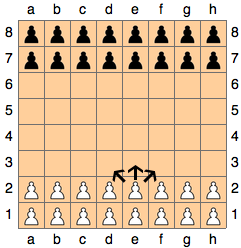
\includegraphics[scale=0.5]{fig1.png}
\caption{Movimento possível da peça e2}
\label{fig:1}
\end{center}
\end{figure}

\item Os jogadores movimentam-se sempre em direção à base do adversário, e nunca podem retroceder.
\item Uma peça pode ser capturada (substituída) se se encontrar diagonalmente ao adversário, quando este avança em direção à base oposta. A captura não é obrigatória nem encadeada como nas damas.

\begin{figure}[H]
\begin{center}
\subfloat[Possibilidades para a peça f3]{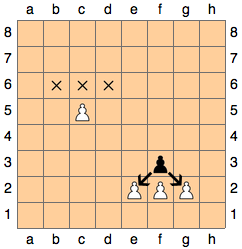
\includegraphics[scale=0.5]{fig2a.png}\label{fig:2a}}\hspace{10px}
\subfloat[Captura de e2]{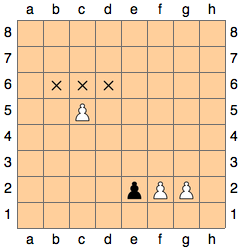
\includegraphics[scale=0.5]{fig2b.png}\label{fig:2b}}
\caption{Processo de captura.}
\label{fig:2}
\end{center}
\end{figure}

\item O primeiro jogador a atingir a base do adversário, vence. No caso anterior, se o jogador preto atingisse a linha 1, venceria.
\item Se todas as peças de um jogador forem capturadas, este perde o jogo.
\item Um empate é matemáticamente impossível, e todas as peças têm sempre pelo menos uma jogada na diagonal possível.

\end{enumerate}


%************************************************************************************************
%************************************************************************************************

\newpage
\section{Representação do Estado do Jogo}
Descrever a forma de representação do estado do tabuleiro (tipicamente uma lista de listas), com exemplificação em Prolog de posições iniciais do jogo, posições intermédias e finais.

\section{Representação de um Movimento}
Descrever a forma de representação dos diversos tipos de jogadas (movimentos) permitidos no jogo. Só é necessário apresentar os cabeçalhos dos predicados que serão utilizados para as diferentes jogadas (que ainda não precisam de estar implementados).

\section{Visualização do Tabuleiro}
Descrever a forma de visualização do tabuleiro em modo de texto e os predicados Prolog construídos para o efeito. O código (predicado) desenvolvido, deve receber como parâmetro a representação do tabuleiro (estado do jogo) e permitir visualizar, no ecrã, em modo de texto, o estado do jogo. Deve ser incluída no relatório, pelo menos, uma imagem demonstrando a visualização em modo de texto do tabuleiro.

\section{Conclusões e Perspectivas de Desenvolvimento}
Que conclui da análise do jogo e da pesquisa bibliográfica realizada? Como vai ser desenvolvido o trabalho? Que parte (\%) do trabalho estima que falta fazer?

\clearpage
\addcontentsline{toc}{section}{Bibliografia}
\renewcommand\refname{Bibliografia}
\bibliographystyle{plain}
\bibliography{myrefs}


%************************************************************************************************
%************************************************************************************************

\newpage

\appendix
\section{Nome do Anexo A}
Código Prolog implementado (representação do estado, cabeçalhos dos predicados de jogada e predicado que permite a visualização simples, em modo de texto, do tabuleiro).

\end{document}
